%------------------------------------------------------------------------------
\section{DNS-Server}
%------------------------------------------------------------------------------
Das \textit{Domain Name System} – DNS ist einer der wichtigsten Dienste im
Internet. DNS wird von vielen Diensten wie bspw. Mail und Web-Diensten
verwendet. Neben der Aufgabe menschenlesbare Namen in maschinenlesbare
IP-Adressen aufzulösen, liefert DNS auch wichtige Funktionen um Redundanzen
herzustellen. DNS "`abstrahiert"' Layer-3 Adressen auf einen Namen, damit ist es
möglich, dass weltweit erreichbare Web-Dienste von IP-Adressen unabhängig
werden. DNS ist damit ein wichtiger Bestandteil zur Einführung und
Implementierung von Internetdiensten in Unternehmensnetzen.

%------------------------------------------------------------------------------
\subsection{Installation und Konfiguration von BIND}
%------------------------------------------------------------------------------
Im Internet wird zum großen Teil der quelloffene DNS-Server
\textit{BIND}\footnote{Berkeley Internet Name
Domain: \url{http://www.isc.org/software/bind}} eingesetzt. Im Folgenden wird
der Server \textit{srv200} als Nameserver konfiguriert. Hier wird wieder
exemplarisch die Konfiguration von \textit{srv200} wiedergegeben. Die für Sie
benötigten Werte entnehmen Sie bitte aus der Tabelle im Anhang. Melden Sie sich
wieder am Server \textit{srv200} mit den bekannten Zugangsdaten an. Danach wird
nun die Software \textit{BIND} installiert.

\begin{lstlisting}
admin1@srv200$ sudo aptitude install bind9
\end{lstlisting}

Nach der Installation können wir nun die DNS-Zone konfigurieren:
\begin{lstlisting}
admin1@srv200$ sudo vi /etc/bind/named.conf.options
\end{lstlisting}
Die Datei sollte folgenden Inhalt aufweisen:
\begin{scriptsize}
\begin{lstlisting}
options {
    directory "/var/cache/bind";

    // If there is a firewall between you and nameservers you want
    // to talk to, you may need to fix the firewall to allow multiple
    // ports to talk.  See http://www.kb.cert.org/vuls/id/800113
  
    // If your ISP provided one or more IP addresses for stable 
    // nameservers, you probably want to use them as forwarders.  
    // Uncomment the following block, and insert the addresses replacing
    // the all-0's placeholder.

    forwarders {
      10.174.26.126;
    };

    auth-nxdomain no;    # conform to RFC1035
    listen-on-v6 { any; };
};
\end{lstlisting}
\end{scriptsize}

Damit werden Anfragen, die durch den lokalen Nameserver nicht auflösbar sind an den übergeordneten weitergegeben.

Die Konfiguration von eigenen DNS-Zonen wird zur leichteren Verwaltung und
Administration in drei Dateien vorgenommen:
\begin{itemize}
  \item \texttt{named.conf}: Verweis auf die angelegten Zone-files
  \item \textit{zone.beta.tklabor.site}: Konfiguration der Zone und Verweis auf
  die Zone-DB
  \item \textit{db.beta.tklabor.site}: Zone-DB mit den entsprechenden Einträgen
  für die entsprechende Zone.
\end{itemize}

Die Konfigurationsdateien werden wie folgt verwiesen:

\begin{nofloat}{figure}
	\begin{center}
		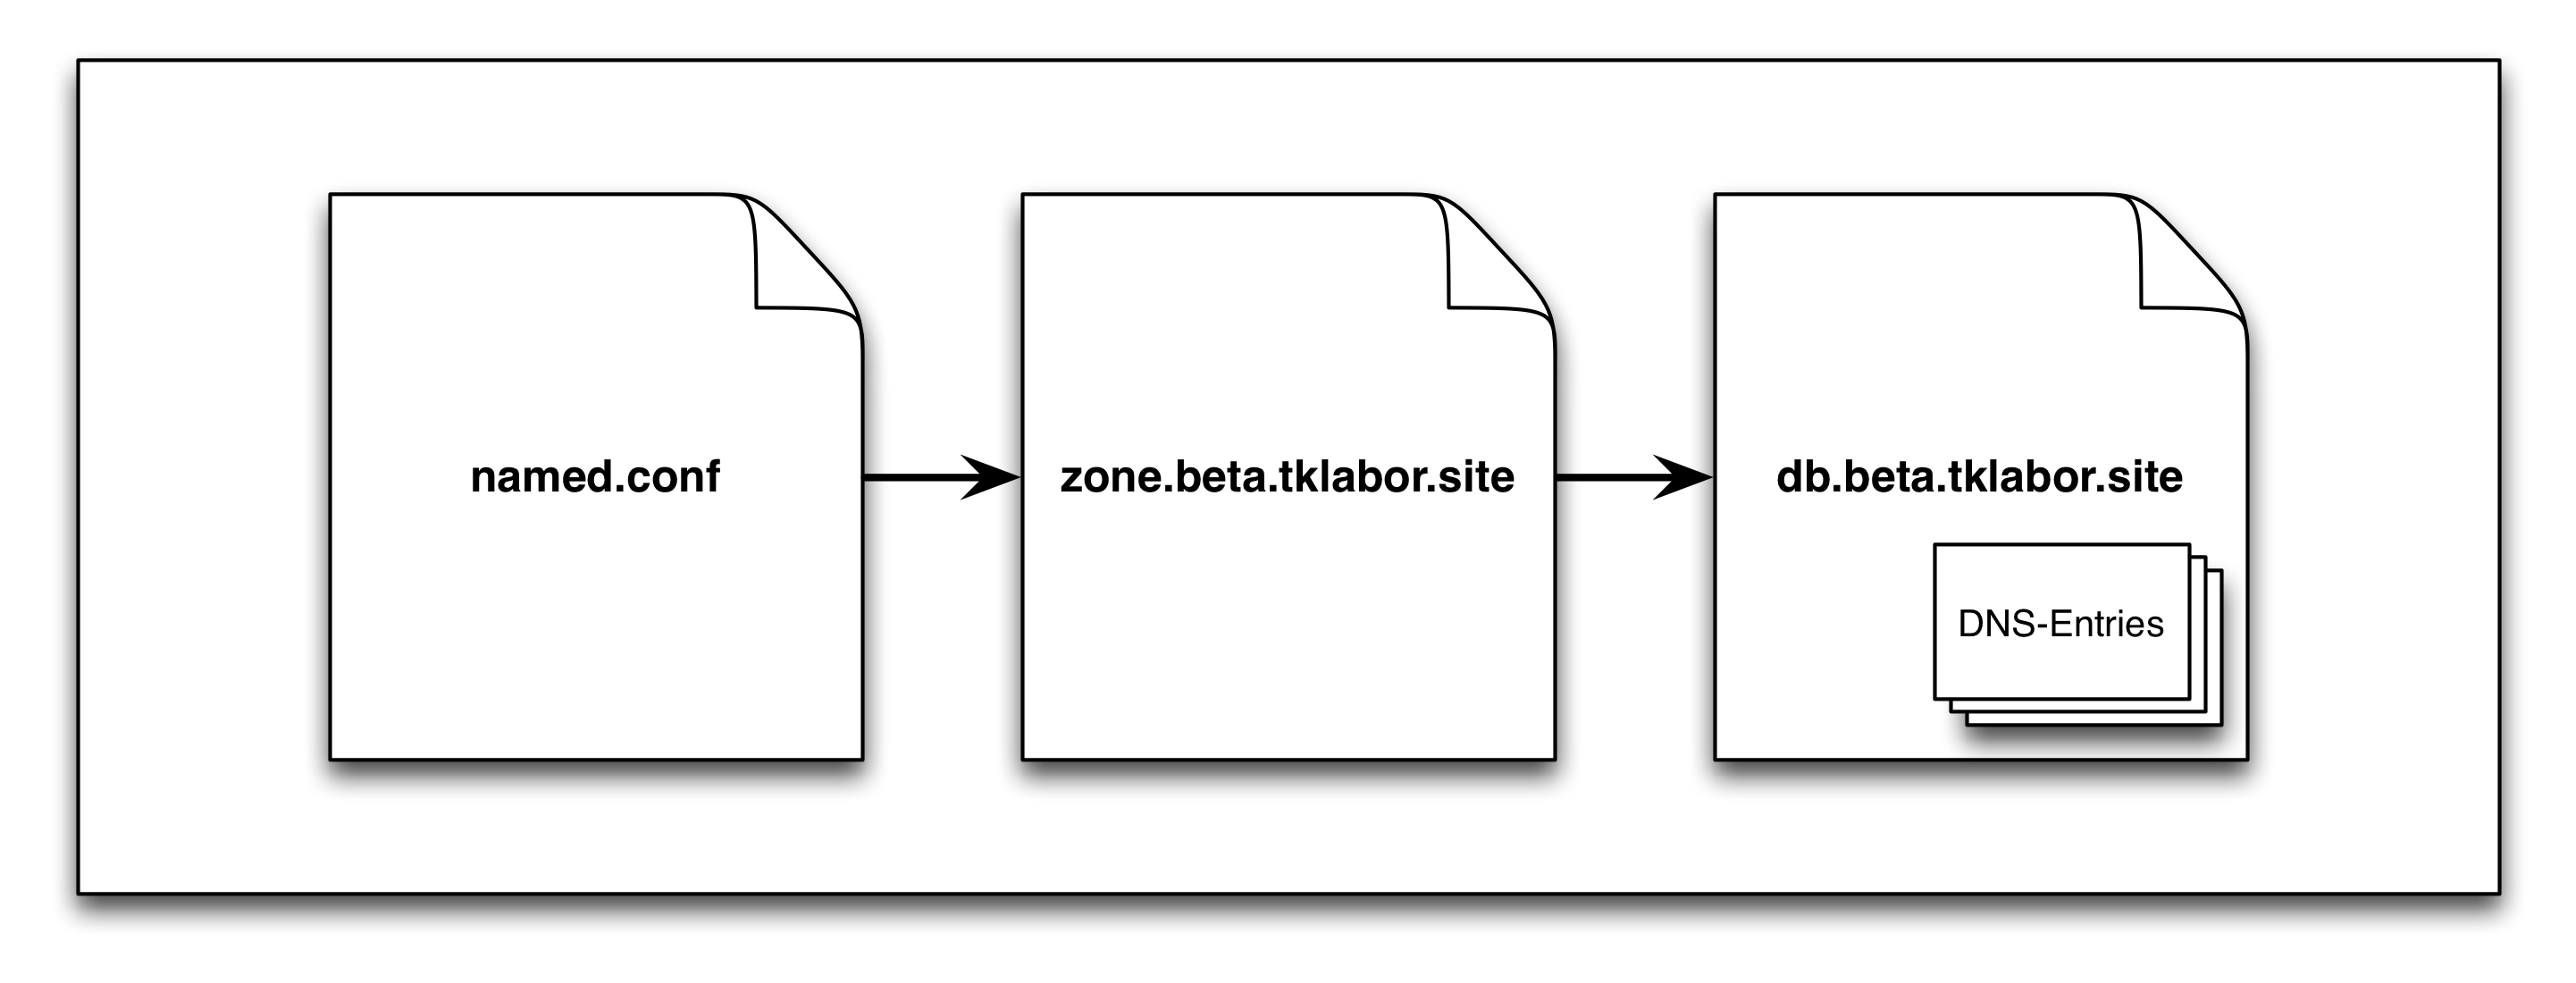
\includegraphics[width=0.85\textwidth]{images/dns-files.png}
	\end{center}
	\caption{Verweiskette der DNS-Zonenkonfiguration}
	\label{fig:bind-config-chain}
\end{nofloat}

Für die Zone \textit{beta.tklabor.site} wird eine Zonendatei erstellt. Diese
Datei wird in der globalen Konfigurationsdatei von \textit{BIND} wie folgt
inkludiert:

\begin{lstlisting}
admin1@srv200$ sudo vi /etc/bind/named.conf
\end{lstlisting}

Diese sollte dann folgendermaßen aussehen:

\begin{scriptsize}
\begin{lstlisting}
// This is the primary configuration file for the BIND DNS server named.
//
// Please read /usr/share/doc/bind9/README.Debian.gz for information on the 
// structure of BIND configuration files in Debian, *BEFORE* you customize 
// this configuration file.
//
// If you are just adding zones, please do that in /etc/bind/named.conf.local

include "/etc/bind/named.conf.options";
include "/etc/bind/named.conf.local";
include "/etc/bind/named.conf.default-zones";
include "/etc/bind/zone.beta.tklabor.site";
\end{lstlisting}
\end{scriptsize}

Für die Zone wird eine Datei \texttt{/etc/bind/zone.beta.tklabor.site}
angelegt.

\begin{lstlisting}
admin1@srv200$ sudo vi /etc/bind/zone.beta.tklabor.site
\end{lstlisting}

\begin{scriptsize}
\begin{lstlisting}
zone "beta.tklabor.site" IN {
	type master;
	file "/etc/bind/db.beta.tklabor.site";
};
\end{lstlisting}
\end{scriptsize}

Im letzten Schritt muss eine Datenbank-Datei für die eigentlichen
Zonen-Einträge erstellt werden:

\begin{lstlisting}
admin1@srv200$ sudo vi /etc/bind/db.beta.tklabor.site
\end{lstlisting}

Diese sollte dann folgenden Inhalt haben:

\begin{scriptsize}
\begin{lstlisting}
$TTL 3600
$ORIGIN beta.tklabor.site.
;
; forward lookup for beta.tklabor.site
;
@    IN   SOA  ns.beta.tklabor.site. root.beta.tklabor.site. ( 
				100		; Serial
				1m		; Refresh
				5m		; Retry
				30d		; Expire
				1h )	; Negative caching TTL
     IN   NS   ns.beta.tklabor.site.
ns   IN   A    10.174.26.200
\end{lstlisting}
\end{scriptsize}

Jetzt stoppen und starten wir den entsprechenden Dienst:
\begin{lstlisting}
admin1@srv200$ sudo service bind9 restart
\end{lstlisting}

Um die Namensauflösung jetzt über den eigenen DNS-Server durchzuführen muss auf
beiden Servern der DNS-Server geändert werden. Die Abfragen werden nun nicht
mehr auf den 10.174.26.126 durchgeführt.
\begin{lstlisting}
admin1@srv200:~$ sudo vi /etc/resolv.conf
\end{lstlisting}

Die Datei sollte dann wie folgt aussehen:
\begin{scriptsize}
\begin{lstlisting}
nameserver 10.174.26.200
domain beta.tklabor.site
search beta.tklabor.site
\end{lstlisting}
\end{scriptsize}

In der Regel sollte es nun möglich sein den Nameserver der Domäne
\textit{beta.tklabor.site} zu ermitteln.

\begin{scriptsize}
\begin{lstlisting}
root@srv200:/etc/bind# dig ns beta.tklabor.site

; <<>> DiG 9.7.1-P2 <<>> ns beta.tklabor.site
;; global options: +cmd
;; Got answer:
;; ->>HEADER<<- opcode: QUERY, status: NOERROR, id: 40508
;; flags: qr aa rd ra; QUERY: 1, ANSWER: 1, AUTHORITY: 0, ADDITIONAL: 1

;; QUESTION SECTION:
;beta.tklabor.site.		IN	NS

;; ANSWER SECTION:
beta.tklabor.site.	3600	IN	NS	ns.beta.tklabor.site.

;; ADDITIONAL SECTION:
ns.beta.tklabor.site.	3600	IN	A	10.174.26.200

;; Query time: 0 msec
;; SERVER: 10.174.26.200#53(10.174.26.200)
;; WHEN: Wed Mar 30 18:17:40 2011
;; MSG SIZE  rcvd: 68
\end{lstlisting}
\end{scriptsize}

\subsection{Aufgabe}
\begin{enumerate}
  \item Welche Bedeutung haben die Einträge der Zonendatei: SOA, TTL, NS, A,
  CNAME, PTR, TXT, AAAA
  \item Beschreiben Sie den Inhalt der Datei \textit{db.beta.tklabor.site}
  \item Tragen Sie in die Zone \textit{beta.tklabor.site} einen Alias
  für srv200 und srv201 ein.
  \item Erstellen Sie einen \textit{Canonical Name Record} für srv201 mit der
  Bezeichnung \textit{www}.
  \item Konfigurieren Sie eine Reverse Lookup Zone für 10.174.26.0/24. Eine
  Zonendatenbankdatei als Beispiel finden Sie im Anhang auf Seite
  \pageref{cfg:bind-reverse-lookup}.
 \end{enumerate}

%------------------------------------------------------------------------------
\subsection{Funktionstest}
%------------------------------------------------------------------------------
Prüfen die folgenden Funktionen:
\begin{enumerate}
  \item Testen Sie die Namensauflösung für srv200.beta.tklabor.site und für
  srv201.beta.tklabor.site
  \item Testen Sie die Namensauflösung für www.beta.tklabor.site
  \item Testen Sie die Namensauflösung einer Internetdomain \textit{www.fsf.org}
  \item Testen Sie den Reverse Lookup für 10.174.26.200 mit \texttt{nslookup}
  und \texttt{dig}
  \item Testen Sie die oben genannte Namensauflösung mit \texttt{dig +trace}.
  \item Wie verhält sich \texttt{dig @10.174.26.126 www.fsf.org} im Gegensatz\\
  zu \texttt{dig @10.174.26.200 www.fsf.org}?
\end{enumerate}

%------------------------------------------------------------------------------
\subsection{DNS Replikation - Zone Transfer}
%------------------------------------------------------------------------------
Die Bereitstellung von Internetdiensten basiert zu einem sehr großen Teil auf
dem DNS-Service. Fällt dieser Dienst aus, kann es vorkommen, dass die Zustellung
von unternehmenskritischen Mails oder Zugriffe auf Web-Portale nicht mehr
möglich sind. Aus diesem Grund kann es Sinnvoll sein DNS-Server redundant
einzurichten. Im folgenden Abschnitt wird auf dem zweiten Server ein DNS-Server
installiert. Er wird die Zone \textit{beta.tklabor.site} als Backup-DNS Server
bereitstellen. Der Server \textit{srv201} wird zu diesem Zweck als \textit{Slave
Nameserver} eingerichtet. Änderungen können zentral auf dem primären DNS-Server
\textit{srv200} vorgenommen werden. Die Einträge werden dann mittels
Zonentransfer auf den Slave-Server automatisch übertragen. Auf dem Server soll
automatisch eine Kopie der Zonendatenbank gespeichert werden. Die Aktualisierung
der Zone soll jede Minute abgeglichen werden.\\
\\
\textbf{\textit{Hinweis}}: In größeren Umgebungen ist der Zonenabgleich sehr
aufwändig und wird daher in 4 Stunden Intervalen aktualisiert. In der
Laborumgebung ist ein kurzer Interval zum Test sinnvoll.

\textbf{\textit{WICHTIG!}}: Bitte ändern Sie auf dem primären DNS-Server den
Parameter \textit{Refresh} der Zone auf \texttt{1m}. 

Für die Einrichtung melden wir uns auf dem Rechner \textit{srv201} als
\textit{admin2} an und installieren \textit{BIND}.

\begin{lstlisting}
admin1@srv201:~$ sudo aptitude install bind9
\end{lstlisting}

Wir richten auf dem Server die Zone \textit{beta.tklabor.site} ein.
\begin{lstlisting}
admin1@srv201:~$ sudo vi /etc/bind/named.conf
\end{lstlisting}
\begin{scriptsize}
\begin{lstlisting}
// This is the primary configuration file for the BIND DNS server named.
//
// Please read /usr/share/doc/bind9/README.Debian.gz for information on the 
// structure of BIND configuration files in Debian, *BEFORE* you customize 
// this configuration file.
//
// If you are just adding zones, please do that in /etc/bind/named.conf.local

include "/etc/bind/named.conf.options";
include "/etc/bind/named.conf.local";
include "/etc/bind/named.conf.default-zones";
include "/etc/bind/zone.beta.tklabor.site";
\end{lstlisting}
\end{scriptsize}

Im nächsten Schritt erstellen wir die Zonendatei. Die Zone ist hier nicht vom
Typ \textit{master} sondern wird als \textit{slave} Zone erstellt. Die
Backupdatei für unsere Zonendatenbank müssen wir nicht angeben, diese wird vom
primären Server repliziert. Die replizierte Datenbank wollen wir uns ebenfalls
als Datei sichern und kennzeichnen sie mit dem Prefix \textit{bak}. Als Quelle
geben den Server \textit{srv200} an.

\begin{scriptsize}
\begin{lstlisting}
zone "beta.tklabor.site" IN {
	type slave;
	file "/var/lib/bind/bak.beta.tklabor.site";
	masters { 10.174.26.200; };
};
\end{lstlisting}
\end{scriptsize}

Um die Konfiguration anzuwenden wird \textit{BIND} neu gestartet.
\begin{lstlisting}
admin1@srv201:~$ sudo service bind9 restart
\end{lstlisting}

%------------------------------------------------------------------------------
\subsection{Funktionstest und Aufgaben}
%------------------------------------------------------------------------------
Prüfen Sie ob die Zonendatenbank in das Verzeichnis kopiert worden ist und ob
entsprechende Einträge vorhanden sind.

\begin{lstlisting}
admin1@srv201:~$ cat /var/lib/bind/bak.beta.tklabor.site
\end{lstlisting}

\begin{enumerate}
  \item Testen Sie mit \texttt{dig @10.174.26.201} ob die DNS-Auflösung
  funktioniert.
  \item Erzeugen Sie einen weiteren \textit{Alias Record} von \textit{ns2} dem
  primären DNS-Server für \textit{srv201}. Erhöhen Sie die \textit{Serial} um
  \texttt{1} und speichern die Änderung ab. Sie können \textit{BIND} dazu
  veranlassen nur die geänderte Zone neu zu laden. Verwenden Sie dazu das
  Kommando: \texttt{rndc reload beta.tklabor.site}. Prüfen Sie die Logdatei auf
  dem Backup-DNS Server mit \texttt{tail -f /var/log/syslog}. Nach einer Minute
  sollte die Änderung repliziert sein.
  \item Testen Sie die Namensauflösung mit \texttt{dig @10.174.26.201} für den
  neuen Eintrag \textit{ns2.beta.tklabor.site}
  \item Stoppen Sie \textit{BIND} auf dem primären Server \textit{srv200} und
  prüfen ob die Namensauflösung noch möglich ist. Anhand welcher Konfiguration
  wird entschieden wie die Namensauflösung durchgeführt wird?
\end{enumerate}

%------------------------------------------------------------------------------
\subsection{Einschränken der Replikation}
%------------------------------------------------------------------------------
Ob eine Replikation von einem bestimmten DNS-Server funktioniert, kann von der
Konsole getestet werden:

\begin{lstlisting}
admin1@srv201:~$ dig @10.174.26.200 beta.tklabor.site AXFR
\end{lstlisting}

\begin{enumerate}
  \item Prüfen Sie, ob von einem beliebigen DNS-Server im Labor die komplette
  Zone auslesen können.
  \item Schränken Sie auf dem primären DNS-Server Ihrer Zone
  \texttt{zone.beta.tklabor.site} mit der Option \texttt{allow-transfer \{ 10.174.26.201; \};} die Abfrage ein.
  \item Prüfen Sie ob ein Zonentransfer auch von Ihrem Slave-Server
  funktioniert. Falls ja verbieten Sie den Zonentransfer von Ihrem Slave-Server
  komplett mit der Option\\ \texttt{allow-transfer \{ none; \};}.
  \item Prüfen Sie mit \texttt{dig} ob Ihre Konfiguration funktioniert.
\end{enumerate}
